\section{Tecnologie}

\subsection{Introduzione}

\begin{frame}{Tecnologie utilizzate}

\begin{itemize}
\item JBoss AS (Application Server) 7.1
	\begin{itemize}
	
	\vspace{0.5em}
	
	\item fornisce l'infrastruttura per consentire l'esecuzione di una web application
	\end{itemize}

\vspace{1em}

\item Java EE (Java Platform, Enterprise Edition) 6
	\begin{itemize}
	
	\vspace{0.5em}
	
	\item piattaforma software per lo sviluppo di applicazioni enterprise
	
	\vspace{0.7em}
	
	\item comprende varie tecnologie, fra cui:
		\begin{itemize}
		
		\vspace{0.4em}
		
		\item JPA (Java Persistence API) 2.0
		
		\vspace{0.6em}
		
		\item CDI (Contexts and Dependency Injection) 1.0
		
		\vspace{0.6em}
		
		\item JSF (JavaServer Faces) 2.0
		\end{itemize}
		
	\end{itemize}

\end{itemize}


\end{frame}

\begin{frame}{Bean}

\begin{itemize}
\item Sono componenti software riusabili che possono essere gestiti dal container

\vspace{1em}

\item Vari tipi:
	\begin{itemize}
	
	\vspace{0.8em}
	
	\item \textsl{Enterprise JavaBeans} (EJB): bean utilizzati per la logica di business o la persistenza
		\begin{itemize}
		
		\vspace{0.5em}
		
		\item session bean
		
		\vspace{0.3em}
		
		\item message-driven bean
		
		\vspace{0.3em}
		
		\item entity bean
		\end{itemize}
	
	\vspace{0.8em}
	
	\item  \textsl{Managed beans}: bean utilizzati a livello di presentazione
	\end{itemize}

\end{itemize}

\end{frame}


\subsection{JPA}
\begin{frame}{Java Persistence API}

\begin{itemize}
\item Si occupa della persistenza dei dati
\end{itemize}

\vspace{0.4em}

\begin{itemize}
\item Problema:

	\begin{itemize}
	
	\vspace{0.4em}

	\item Nelle applicazioni enterprise è necessario ricorrere ad un database
	
	\vspace{0.7em}
	
	\item Database: \textsl{modello relazionale}
		\begin{itemize}
		
		\vspace{0.4em}
		
		\item entità: \textsl{relazioni}
		
		\vspace{0.2em}
		
		\item collegate tra di loro mediante \textsl{chiavi}
		\end{itemize}
		
	\vspace{0.7em}
	
	\item Applicazione Java: \textsl{modello a oggetti}
		\begin{itemize}
		
		\vspace{0.4em}
		
		\item entità: \textsl{classi}
		
		\vspace{0.2em}
		
		\item collegate tra di loro mediante \textsl{riferimenti}
		\end{itemize}
	
	\end{itemize}

\end{itemize}

\end{frame}


\begin{frame}{Integrazione fra i modelli}

\begin{itemize}
\item Occorre un sistema per la conversione tra i due modelli

	\begin{itemize}
	
	\vspace{0.7em}
	
	\item non deve influire pesantemente sullo sviluppo dell'applicazione
	
	\vspace{0.7em}
	
	\item in particolare, deve garantire:
	
		\begin{itemize}
		\item trasparenza rispetto al modello di dominio
		
		\vspace{0.5em}
		
		\item recupero di informazioni indipendente dal database
		
		\vspace{0.5em}
		
		\item compatibilità con database preesistenti
		\end{itemize}
	
	\end{itemize}

\end{itemize}

\end{frame}


\begin{frame}{Costrutti fondamentali}

\begin{itemize}
\item Entità
	\begin{itemize}
	\item è un'unità che possiede uno stato e può essere persistita
	\item una classe Java è un'entità se:
		\begin{itemize}
		\item è annotata \texttt{@Entity}
		\item ha un costruttore senza parametri
		\end{itemize}
	\end{itemize}

\vspace{1em}

\item Entity Manager
	\begin{itemize}
	\item gestisce le entità
	\item è associato ad un \textsl{Persistence Context}
		\begin{itemize}
		\item è l'insieme delle entità gestite da un Entity Manager in un dato momento
		\item se un entità fa parte di un Persistence Context viene detta \textsl{managed}
		\item altrimenti viene detta \textsl{detached}
		\end{itemize}
	\end{itemize}

\end{itemize}	


\end{frame}

\begin{frame}{Query}

\begin{itemize}
\item Si usa il \textsl{Java Persistence Query Language} (JPQL)

\vspace{1em}

\item Sintassi simile a SQL, ma:

	\begin{itemize}
	
	\vspace{0.5em}
	
	\item è indipendente dal database
	
	\vspace{0.8em}
	
	\item utilizza le entità del modello di dominio e relativi attributi
	\end{itemize}


\end{itemize}

\end{frame}


\subsection{CDI}

\begin{frame}{Contexts and Dependency Injection}

\begin{itemize}
\item Problema: incompatibilità tra
	\begin{itemize}
	
	\vspace{0.5em}
	
	\item il livello di business, che usa EJB;
	
	\vspace{0.8em}
	
	\item il livello di presentazione, che usa Managed bean.
	\end{itemize}
	
\vspace{1em}	

\item CDI:
	\begin{itemize}
	
	\vspace{0.5em}
	
	\item consente l'utilizzo di EJB nel livello di presentazione
	
	\vspace{0.8em}
	
	\item fornisce una specifica per la definizione di Managed bean
		\begin{itemize}
		
		\vspace{0.5em}
		
		\item integrazione Expression Language (EL)
		\end{itemize}
	\end{itemize}
\end{itemize}

\end{frame}



\begin{frame}{Contesto}

\begin{itemize}
\item Lo \textsl{scope} di un bean determina:

	\begin{itemize}
	
	\vspace{0.5em}
	
	\item il tempo di vita (\textsl{lifetime})
	
	\vspace{0.8em}
	
	\item la visibilità
	\end{itemize}

\vspace{1em}

\item 4 possibili \textsl{scope}:
	\begin{itemize}
	
	\vspace{0.5em}
	
	\item Request
	
	\vspace{0.8em}
	
	\item Conversation
	
	\vspace{0.8em}
	
	\item Session
	
	\vspace{0.8em}
	
	\item Application
	\end{itemize}

\end{itemize}

\end{frame}



\begin{frame}{Iniezione di dipendenza}

\begin{itemize}
\item Forte controllo sui tipi

\vspace{1em}

\item Scelta della dipendenza:

	\begin{itemize}
	
	\vspace{0.5em}
	
	\item in fase di sviluppo
	
	\vspace{0.8em}
	
	\item in fase di deploy
	
	\vspace{0.8em}
	
	\item a runtime
	
	\end{itemize}



\end{itemize}

\end{frame}


\subsection{JSF}

\begin{frame}{JavaServer Faces}

\begin{itemize}
\item Framework per lo sviluppo di interfaccia grafica

\vspace{0.8em}

\item \textsl{Component-based}

\vspace{0.8em}

\item Consente estensione delle funzionalità tramite librerie di terze parti
\end{itemize}

\end{frame}


\begin{frame}{Architettura}

\begin{itemize}
\item Architettura Model-View-Controller
\end{itemize}

\begin{figure}
	\centering
	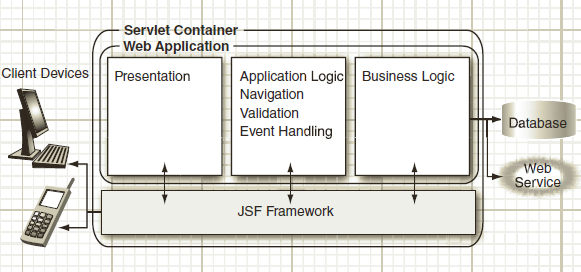
\includegraphics[width=0.5\textwidth]{JSF_architecture.png}
\end{figure}

\end{frame}


\begin{frame}{Comunicazione client-server}
\begin{figure}
	\centering
	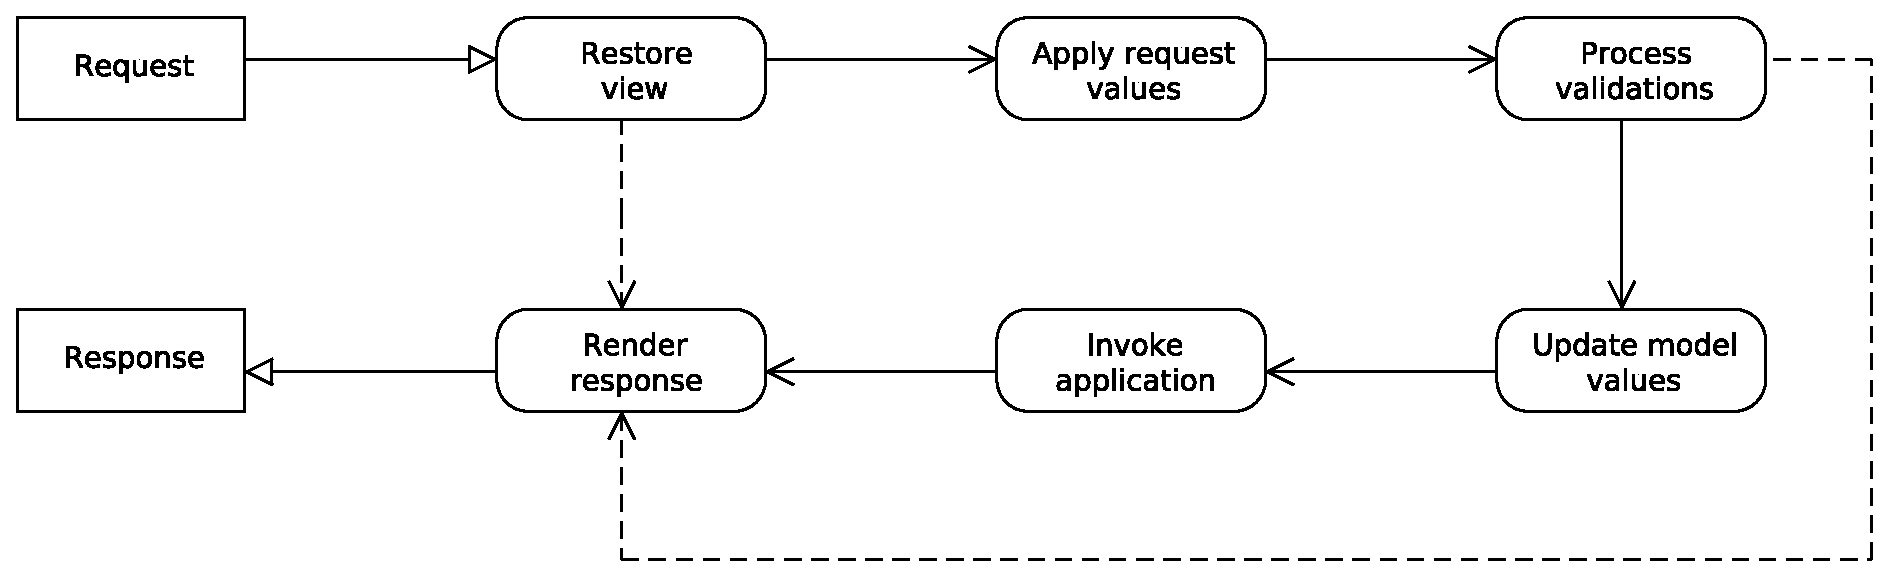
\includegraphics[width=1\textwidth]{custom_JSF_lifecycle.eps}
\end{figure}

\end{frame}


\subsection{Architettura}

\begin{frame}{Architettura tecnologie}
\begin{figure}
	\centering
	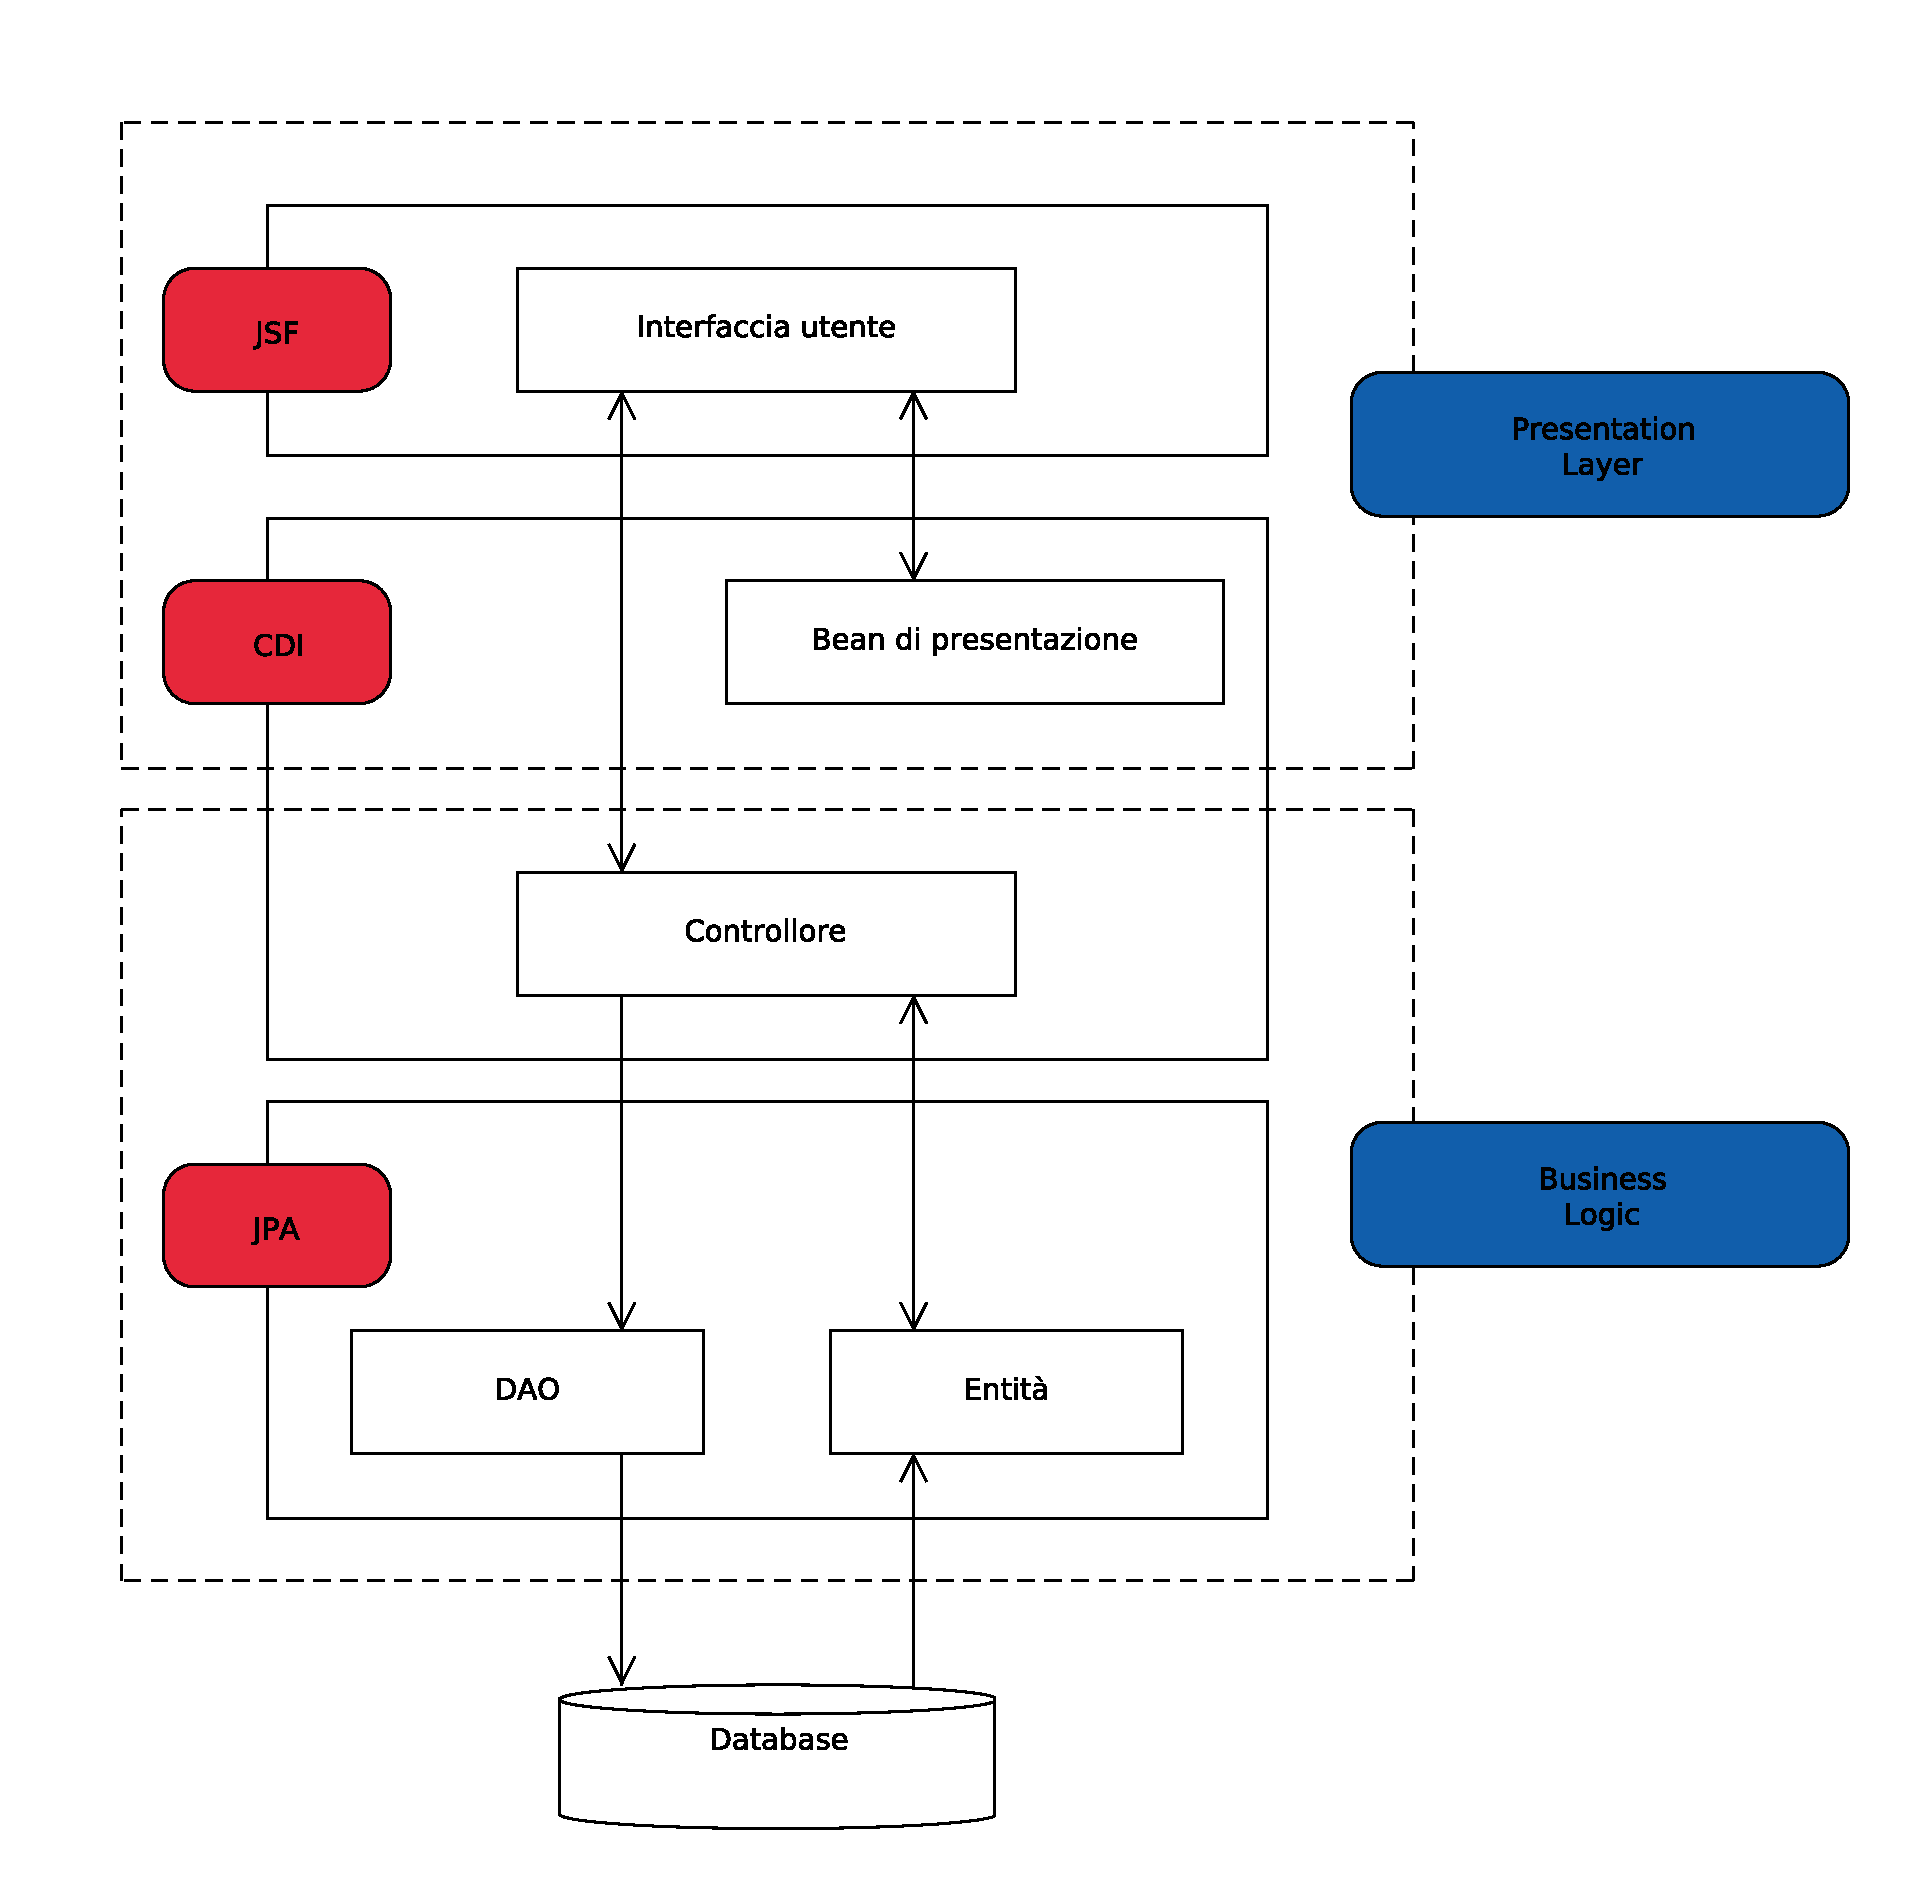
\includegraphics[width=0.6\textwidth]{tech_architecture.eps}
\end{figure}
\end{frame}



